\documentclass[12pt]{article}

 %% preamble
 \usepackage[utf8]{inputenc}
 \usepackage{graphicx}
 \usepackage{booktabs}
 \usepackage{amsmath}
 \usepackage{natbib}
 \usepackage{float}
 \usepackage[colorlinks=true, citecolor=blue]{hyperref}
 \usepackage{bookmark}


 %% meta data

 \title{How Different Variables Affect Depression Scores in Individuals, and Which Set of Variables Provide the Best Outcomes}
 \author{Olivia Dybinski\\}
 \date{November 2022}

 \begin{document}
 \maketitle


 \section{Abstract} 
 \label{sec:abstract}

 This paper will take a look at various variables and see how they affect the percent change of depression scores from before therapy and after therapy. Depression affects millions worldwide, and taking a look at which specific parameters allow for music therapy to be the most beneficial can help guide individuals in the right direction when looking to improve their depression. Some variables considered were individual vs group therapy, total time in therapy, age of participants, and active vs receptive therapy.

 \section{Keywords}
 \label{sec:keywords}

 active music therapy, depression, group music therapy, individual music therapy, instruments, music therapy, receptive music therapy, singing

 \section{Introduction} 
 \label{sec:introduction}

 Depression affects more than 300 million people worldwide and is a large cause of death due to it being closely related to suicide \citet{PLOS}. Depression is defined as a mood disorder that consists of persistent low mood, loss of interest, and a loss of pleasure \citet{Cochrane}. It is the second leading cause of death with almost 800,000 people dying of depression every year worldwide \citet{PLOS}. 

 There are countless methods out there to try to keep depression at bay, like different kinds of drugs, different kinds of therapy, and other programs. Sometimes it can be difficult for those without access to some of these methods to be treated for depression, so it is important to have treatments available that do not involve prescription medications or therapists. Music is something that has been passed down for generations, and is more readily accessible than other methods of treating depression, which is why there is a lot of research going into this topic. There have been many other studies done on music therapy. Some include comparing music therapy to traditional methods of treating depression, like psychological, pharmacological, and other therapies \citet{Cochrane}, studies looking at how traditional methods work hand in hand with music therapy \citet{British}, and studies analyzing how music therapy affects a variety of psychosocial practices like arousal, mood, social connection, as well as many others \citet{Frontiers}. All of these studies focus on how music therapy works hand in hand with other therapies or how they affect specific parts of someone, but this analysis focuses on whether or not different variables affect depression in a positive or negative way, and which variables yield the best results. 

 Specifically, the data collected had various variables about the study taken note of, such as if the therapy was individual or group, active or receptive, the average age of participants and how much time was spent total in therapy throughout the sessions. Finding out which variables are more likely to yield better results will aid in figuring out treatment options and treatment plans for people looking to work their depression.

 Section \ref{sec:data} will provide details about the data, and then section \ref{sec:application} will provide all the outputs and explanations for what it all means in terms of depression score. Finally, section \ref{sec:discussion} will provide some closing statements, and how this research could be improved even further. The references are listed at the very end.

 \section{Data} 
 \label{sec:data}

 The data used was collected from several different studies and compiled together in order to form a more cohesive understanding of whether music therapy affects people or not. It is part of an article called: “Effects of Music Therapy on Depression: A Meta-Analysis of Random Controlled Trials” in the National Library of Medicine \citet{PLOS}. 

 The control group in each of these studies was not receiving any sort of music therapy, but the test group was. These were all randomized controlled trials, and a depression scale was used for each one. Each study did not follow the same scale, but the depression scores before vs after are proportional to one another. 
 
 There were two authors that searched through possible papers to find data that met all the criteria to then be compiled into a master document. Since there is data from so many different studies, the data this paper will utilize is an average of the participants in that specific study. So the depression score before and the depression scores after are the averages for the all of the people that participated in that one study. 
 
 There were a couple of specifics that the two authors were looking for when searching for eligible papers and data to compile. They looked for characteristics of the paper, characteristics of the participants, the study design, the music therapy process, and the outcome measures. There are a lot of specifics under those branches that they had in their large data set, but I narrowed it down to the ones that I wanted to focus on, which were the type of music therapy (individual or group), the total number of minutes spent in music therapy over the course of the study/treatment, whether the music therapy was active or receptive, the mean age of the participants, and the depression score before and after treatment. 
 
 They ultimately ended up with 55 studies, 24 of them had the relevant information I was looking for.  Some of the studies did not take note of some of the variables that I wanted to look at, so they were not included. These are some of the variables focused on here: Individual therapy meant they were participating in therapy by themselves rather than with a group. Active therapy means that the individual was actively doing something for their music therapy, which can look like playing an instrument or singing. Receptive therapy is when someone is just absorbing whatever is put in front of them, such as listening to music and lyric analysis. 
 
 The research question I chose to look at is: how do different variables affect how effective music therapy is for individuals with depression, and does music therapy have an overall positive effect on depression? This data set gives me a lot of different variables to look at and compare to the depression scores given. Since there is a test group as well as a control group, I can compare the depression scores before and after for both groups, and see whether the music therapy was actually effective or if the depression score just naturally went down with time.

 \section{Application} 
 \label{sec:application}

 \begin{table}[hbt!]
    \small
    \caption{Test Group Data}
    \label{tab:1}
  \centering
  \begin{tabular}{rrr}
      \toprule
  Depression Score (Before) & Depression Score (After) & Percent Change of Depression Score \\ 
    \midrule
     5.05 & 3.6 & 28.71\\ 
     8 & 5.2 & 35\\ 
     13.1 & 7.9 & 39.69\\ 
     4.1 & 2.1 & 48.78\\ 
     4.17 & 1.38 & 66.91\\ 
     15.52 & 9.82 & 36.73\\  
     5.1 & 3.7 & 27.45\\
     13.34 & 2.81 & 78.94\\
     20.6 & 15.03 & 27.04\\
     12.333 & 11.867 & 3.78\\
     17.39 & 8.22 & 52.73\\
     24.6 & 14.1 & 42.68\\
     5.1 & 2.5 & 50.98\\
     8.13 & 7.16 & 11.93\\
     16.7 & 8.9 & 46.71\\
     17.3 & 7.7 & 55.49\\
     4.2 & 3.9 & 7.14\\
     15.84 & 13.31 & 15.97\\
     14.68 & 12.23 & 16.69\\
     15.7 & 6.3 & 59.87\\
     20.77 & 15.22 & 26.72\\
     8 & 7.2 & 10\\
     7.93 & 7.4 & 6.68\\
     25.22 & 20.78 & 17.61\\
     \bottomrule
  \end{tabular}
  \end{table}
  
  
  \begin{table}[h!]
    \small
    \caption{Control Group Data}
    \label{tab:2}
  \centering
  \begin{tabular}{rrr}
      \toprule
  Depression Score (Before) & Depression Score (After) & Percent Change of Depression Score \\ 
    \midrule
     4.92 & 4.84 & 1.63\\ 
     8 & 6.5 & 18.75\\ 
     13.4 & 15.8 & -17.91\\ 
     1.8 & 2 & -11.11\\ 
     4.23 & 4.15 & 1.89\\ 
     15.03 & 15.53 & -3.33\\  
     7.1 & 5.6 & 21.13\\
     11 & 8.85 & 19.55\\
     20.43 & 21.47 & -5.09\\
     13.353 & 14.559 & -9.03\\
     15.7 & 13.78 & 12.23\\
     23 & 16.43 & 28.57\\
     7.5 & 6 & 20\\
     8.5 & 9.13 & -7.41\\
     11.8 & 11.2 & 5.08\\
     15.3 & 16.2 & -5.88\\
     3.7 & 3.4 & 8.11\\
     15.75 & 15.65 & 0.63\\
     12.73 & 13.04 & -2.44\\
     16 & 10.2 & 36.25\\
     19.56 & 18.05 & 8.14\\
     7.8 & 8.3 & -6.41\\
     10.14 & 8.5 & 16.17\\
     21.13 & 19.31 & 8.61\\
     \bottomrule
  \end{tabular}
  \end{table}

  \begin{figure}[h!]
    \centering
    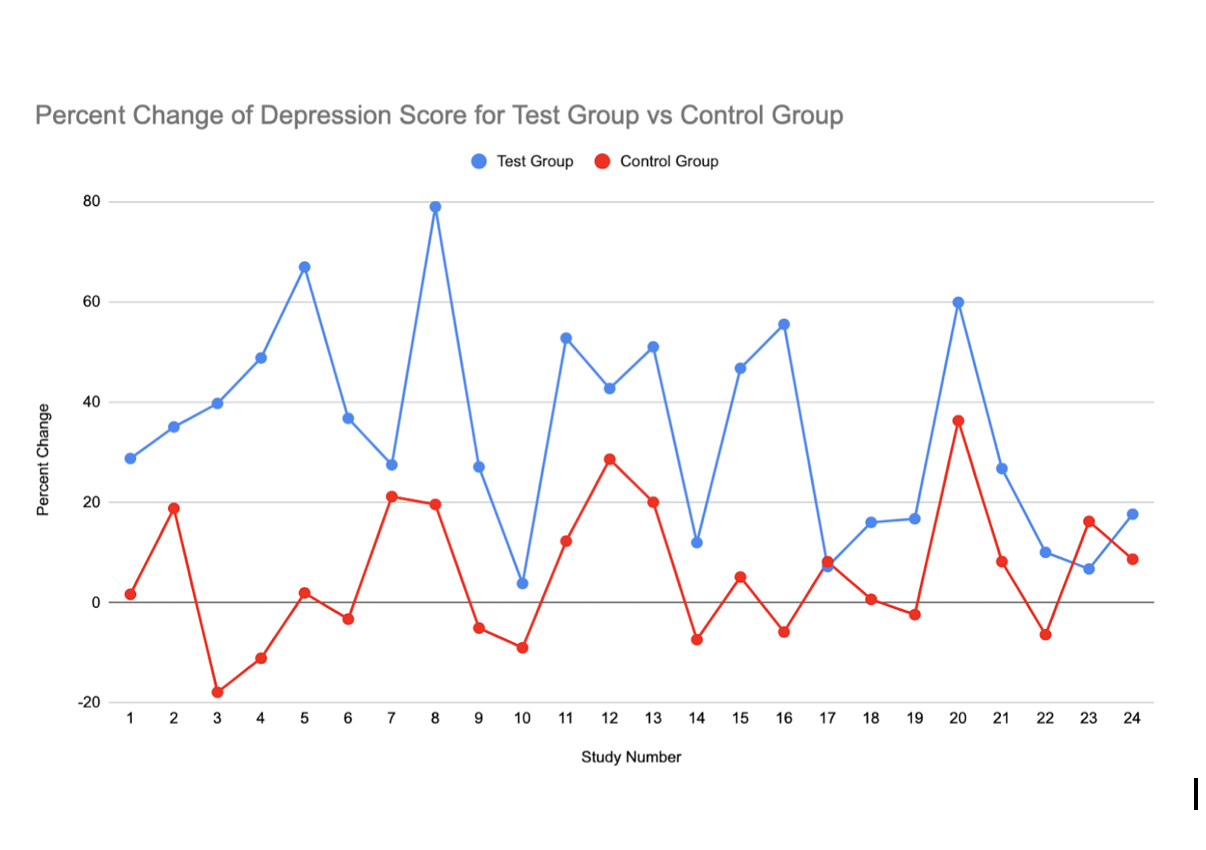
\includegraphics[width=14cm]{CHART1.png}
    \label{fig:chart1}
    \caption{Chart 1}
  \end{figure}


 \begin{samepage}
 The data collected for the depression scores before the therapy started, vs after the therapy started were not in the same scale for each of the studies, as shown in Table 1. Therefore, it did not make sense to compare the difference in scores, or look at the scores directly, because there would most likely be no correlation, since the values range from pretty high to pretty low. Regardless, the percent change looks at the first value of the depression score, the second value of the depression score, and sees by what percentage the score got better or worse. The higher the percent change, the more effective therapy was because the depression score got lower by that percentage. Therefore, a negative percent change means that the depression score after therapy was higher than the depression score before therapy, which means that as time passed the depression got worse. Looking at this graph, the percent change for the test group is higher than the control group in almost every single study, excluding studies 17 and 23. This shows that music therapy was more effective in decreasing depression levels than not having music therapy.
 \end{samepage}

 \begin{figure}[h!]
  \centering
  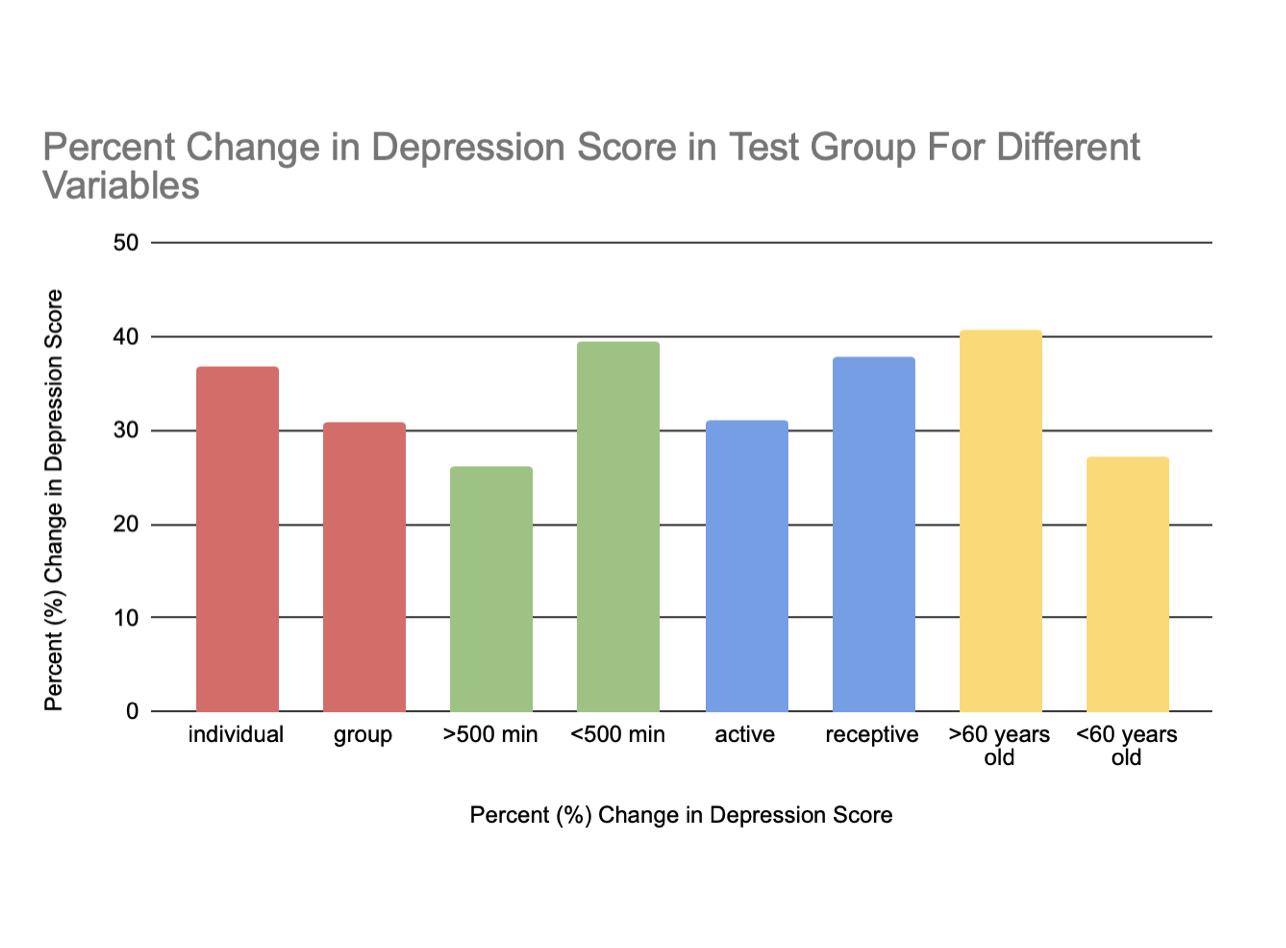
\includegraphics[width=14cm]{CHART2.png}
  \label{fig:chart2}
  \caption{Chart 2}
\end{figure}

 One of the goals with using this data was to compare how different variables affect the depression score, and what set of conditions are the best for making sure that music therapy is most effective. Looking at the first two variables: individual versus group therapy. Individual therapy meant that the patient was participating in the music therapy by themselves, and group therapy meant they were in a group setting participating in the music therapy. The average of the percent change for individual therapy was 36.88\%, which is higher than for group therapy (30.97\%), which means that individual music therapy was more effective in bringing the depression score down than group therapy was. 
 
 The next set of variables was the amount of time that the individual spent total in therapy, and I split the data into two groups, one being $>500$ minutes and the other being $<500$ minutes. I was shocked to see that the set of studies with therapy lasting $<500$ min had a higher average percent change (39.10\%) in depression score than total therapy time being $>500$ min (26.10\%), because it means that more time participating in something does not always yield better results. 
 
 The next variable was whether the individual was active or receptive in their therapy. Active music therapy could include playing instruments, singing, and receptive music therapy could include lyric analysis and listening to music. The graph shows that participating in receptive therapy was more beneficial, as the percent change in depression (37.81\%) was higher  for this group vs the active therapy group (31.15\%). 
 
 The last factor that I looked at was the age of the participants. The patients who were older than 65 $(>65)$ were more receptive to the music therapy than those younger than 65 $(<65)$, as their percent change in depression score is higher (40.67\% vs 27.19\%). Many people think that once an older adult has an issue, it is harder to treat it, but this study just shows that this specific kind of therapy works best on older individuals.

 \begin{figure}[hbt!]
  \centering
  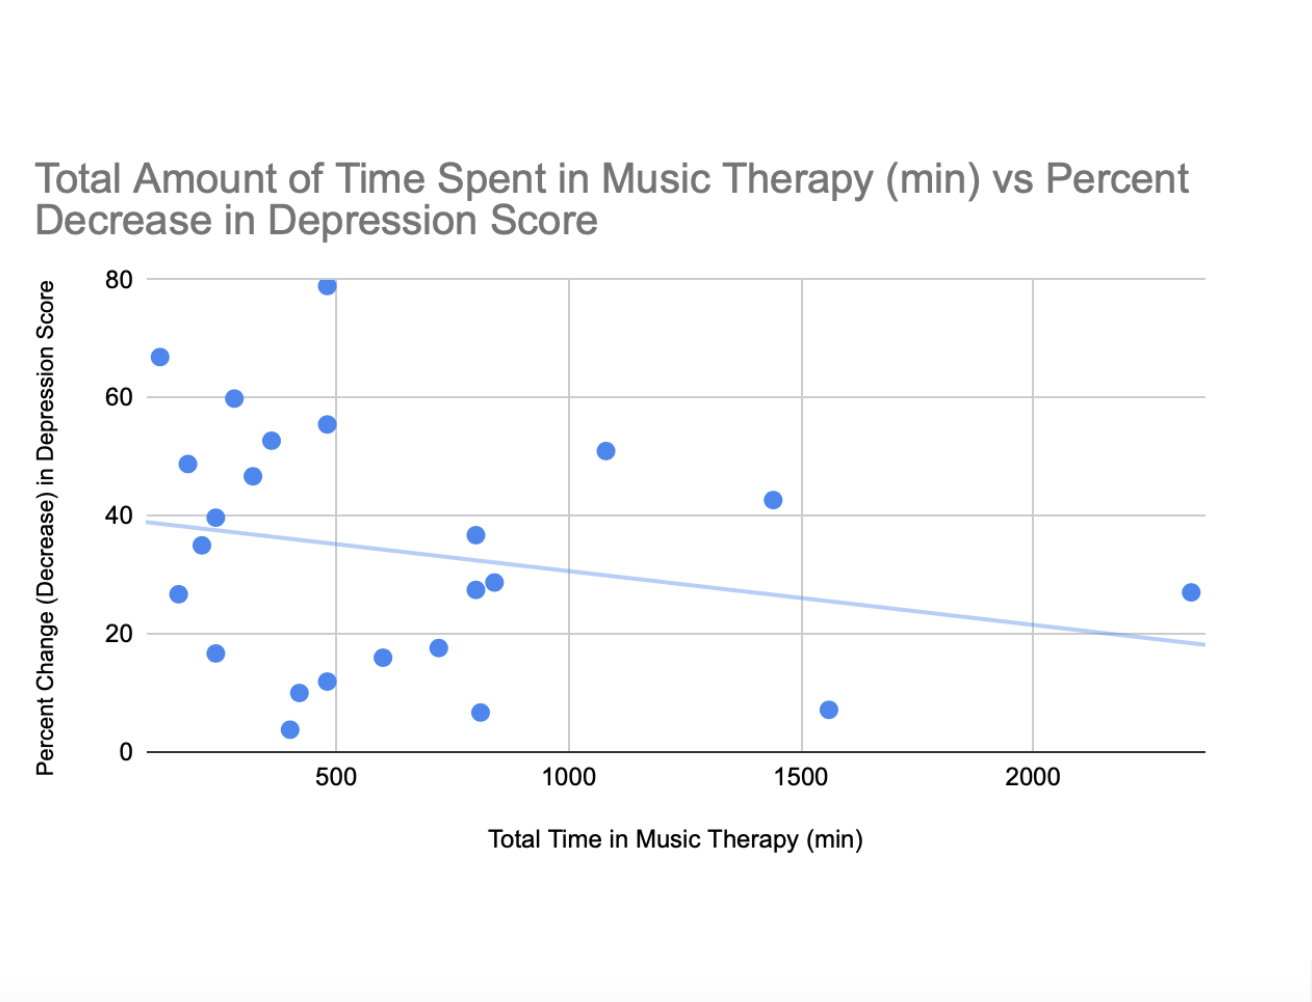
\includegraphics[width=14cm]{CHART3.png}
  \label{fig:chart3}
  \caption{Chart 3}
\end{figure}

 This graph shows the correlation between the total amount of time spent in music therapy and the percent decrease in depression score. There was only one study that had more than 2000 minutes of total time in therapy, which kind of skews the graph. Most of the studies had between 100 and 1000 minutes, and it looks like between 0 and 500 minutes is the ideal amount of time to spend in music therapy in order to see results because the percent change (decrease) in depression scores were highest with that time frame. The more time spent total though, the less intense the percent change was, meaning the depression score did not change as drastically. 

 \section{Discussion} 
 \label{sec:discussion}

 This study allows for individuals looking to see if music therapy is an option for them, which criteria they should aim for in order to have the best outcome. There are obviously more factors that come into play than just the couple that were focused on here, but it is a good starting point. There could be more studies done in the future with even more variables taken into consideration, in order to find the absolute best way to participate in music therapy.


 \bibliographystyle{chicago}
 \bibliography{STAT_W_Paper_cit}{}


\end{document}